\documentclass[a4paper, landscape]{article}
\usepackage{lmodern}
\usepackage{amssymb,amsmath}
\usepackage{ifxetex,ifluatex}
\usepackage{fixltx2e} % provides \textsubscript
\ifnum 0\ifxetex 1\fi\ifluatex 1\fi=0 % if pdftex
  \usepackage[T1]{fontenc}
  \usepackage[utf8]{inputenc}
\else % if luatex or xelatex
  \ifxetex
    \usepackage{mathspec}
    \usepackage{xltxtra,xunicode}
  \else
    \usepackage{fontspec}
  \fi
  \defaultfontfeatures{Mapping=tex-text,Scale=MatchLowercase}
  \newcommand{\euro}{€}
\fi
% use upquote if available, for straight quotes in verbatim environments
\IfFileExists{upquote.sty}{\usepackage{upquote}}{}
% use microtype if available
\IfFileExists{microtype.sty}{%
\usepackage{microtype}
\UseMicrotypeSet[protrusion]{basicmath} % disable protrusion for tt fonts
}{}
\usepackage[margin=0.5cm]{geometry}
\ifxetex
  \usepackage[setpagesize=false, % page size defined by xetex
              unicode=false, % unicode breaks when used with xetex
              xetex]{hyperref}
\else
  \usepackage[unicode=true]{hyperref}
\fi
\hypersetup{breaklinks=true,
            bookmarks=true,
            pdfauthor={pm},
            pdftitle={Descriptions},
            colorlinks=true,
            citecolor=blue,
            urlcolor=blue,
            linkcolor=magenta,
            pdfborder={0 0 0}}
\urlstyle{same}  % don't use monospace font for urls
\usepackage{graphicx,grffile}
\makeatletter
\def\maxwidth{\ifdim\Gin@nat@width>\linewidth\linewidth\else\Gin@nat@width\fi}
\def\maxheight{\ifdim\Gin@nat@height>\textheight\textheight\else\Gin@nat@height\fi}
\makeatother
% Scale images if necessary, so that they will not overflow the page
% margins by default, and it is still possible to overwrite the defaults
% using explicit options in \includegraphics[width, height, ...]{}
\setkeys{Gin}{width=\maxwidth,height=\maxheight,keepaspectratio}
\setlength{\parindent}{0pt}
\setlength{\parskip}{6pt plus 2pt minus 1pt}
\setlength{\emergencystretch}{3em}  % prevent overfull lines
\providecommand{\tightlist}{%
  \setlength{\itemsep}{0pt}\setlength{\parskip}{0pt}}
\setcounter{secnumdepth}{0}

%%% Use protect on footnotes to avoid problems with footnotes in titles
\let\rmarkdownfootnote\footnote%
\def\footnote{\protect\rmarkdownfootnote}

%%% Change title format to be more compact
\usepackage{titling}

% Create subtitle command for use in maketitle
\newcommand{\subtitle}[1]{
  \posttitle{
    \begin{center}\large#1\end{center}
    }
}

\setlength{\droptitle}{-2em}
  \title{Descriptions}
  \pretitle{\vspace{\droptitle}\centering\huge}
  \posttitle{\par}
  \author{pm}
  \preauthor{\centering\large\emph}
  \postauthor{\par}
  \predate{\centering\large\emph}
  \postdate{\par}
  \date{2015-10-27 12:14:54}


% Redefines (sub)paragraphs to behave more like sections
\ifx\paragraph\undefined\else
\let\oldparagraph\paragraph
\renewcommand{\paragraph}[1]{\oldparagraph{#1}\mbox{}}
\fi
\ifx\subparagraph\undefined\else
\let\oldsubparagraph\subparagraph
\renewcommand{\subparagraph}[1]{\oldsubparagraph{#1}\mbox{}}
\fi

\begin{document}
\maketitle

\pagebreak{}

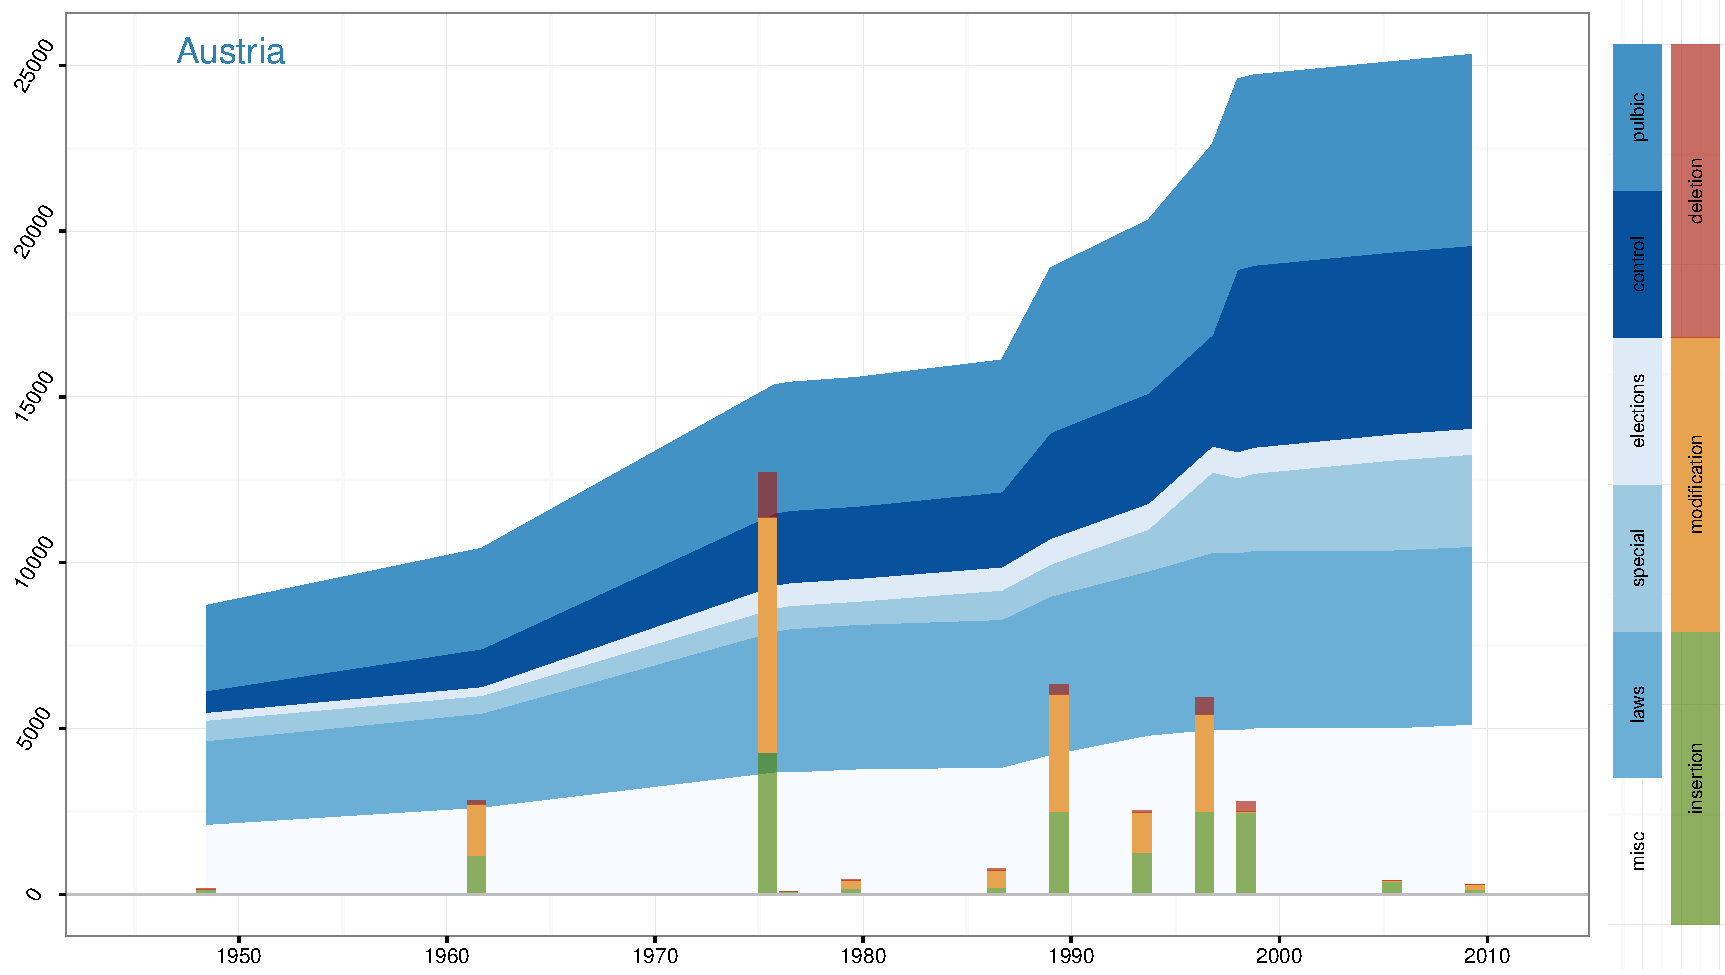
\includegraphics{country_graphs_files/figure-latex/unnamed-chunk-3-1.pdf}
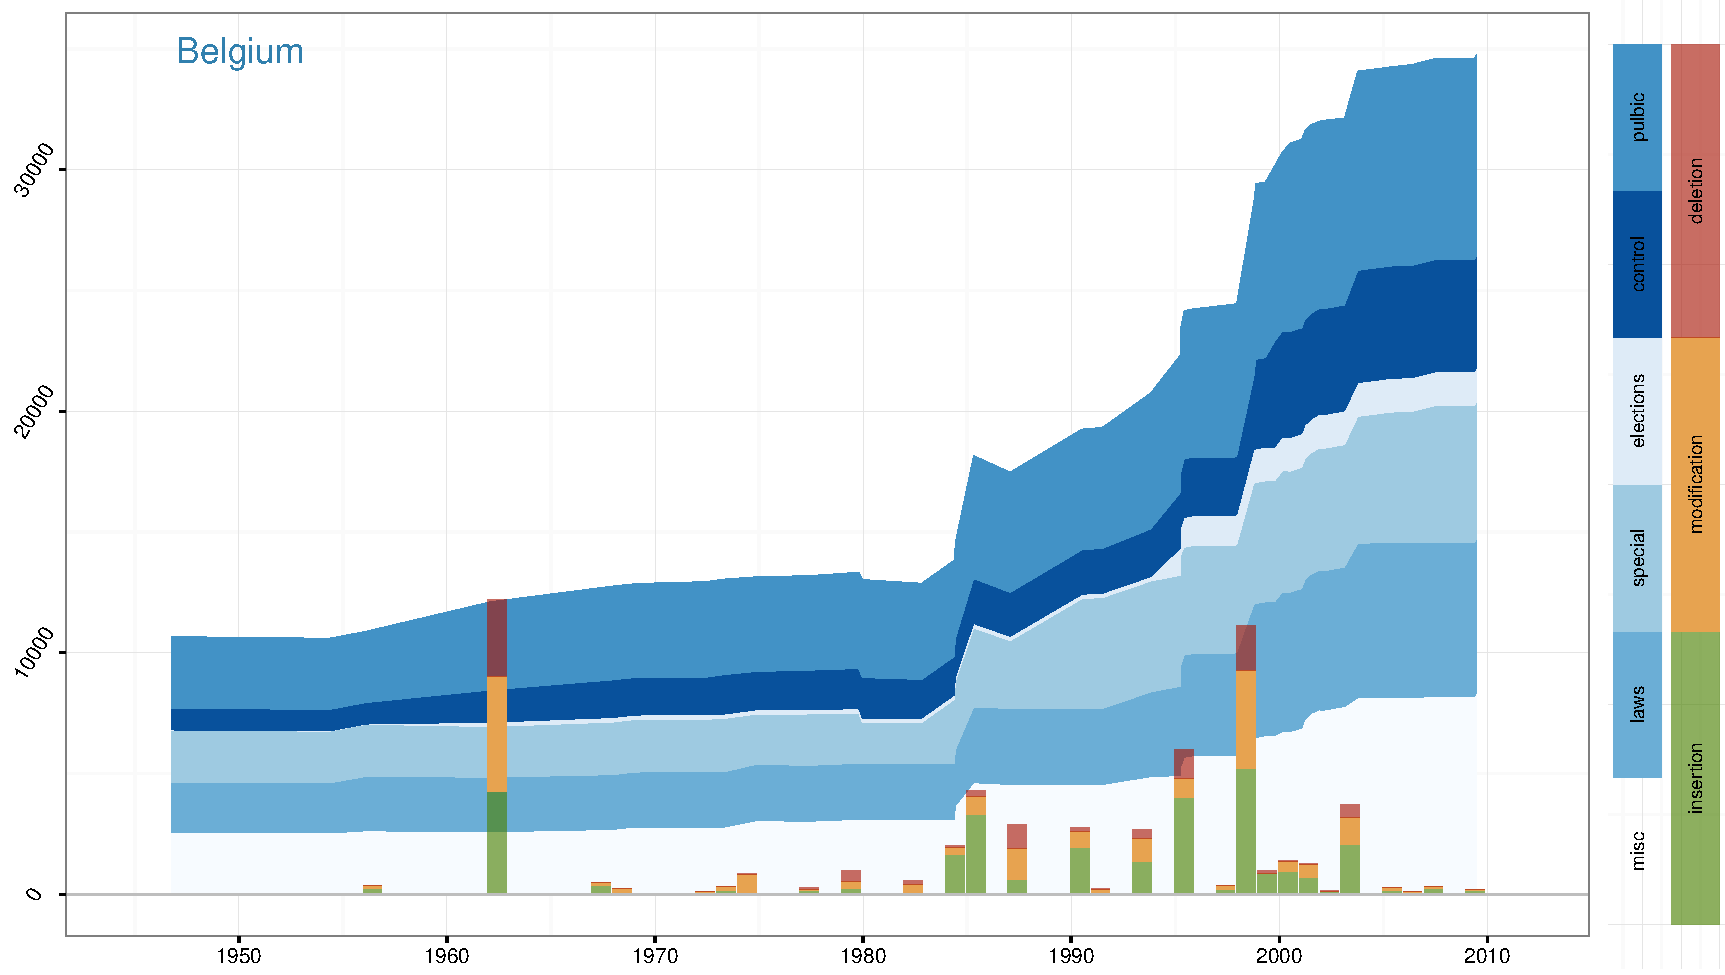
\includegraphics{country_graphs_files/figure-latex/unnamed-chunk-3-2.pdf}
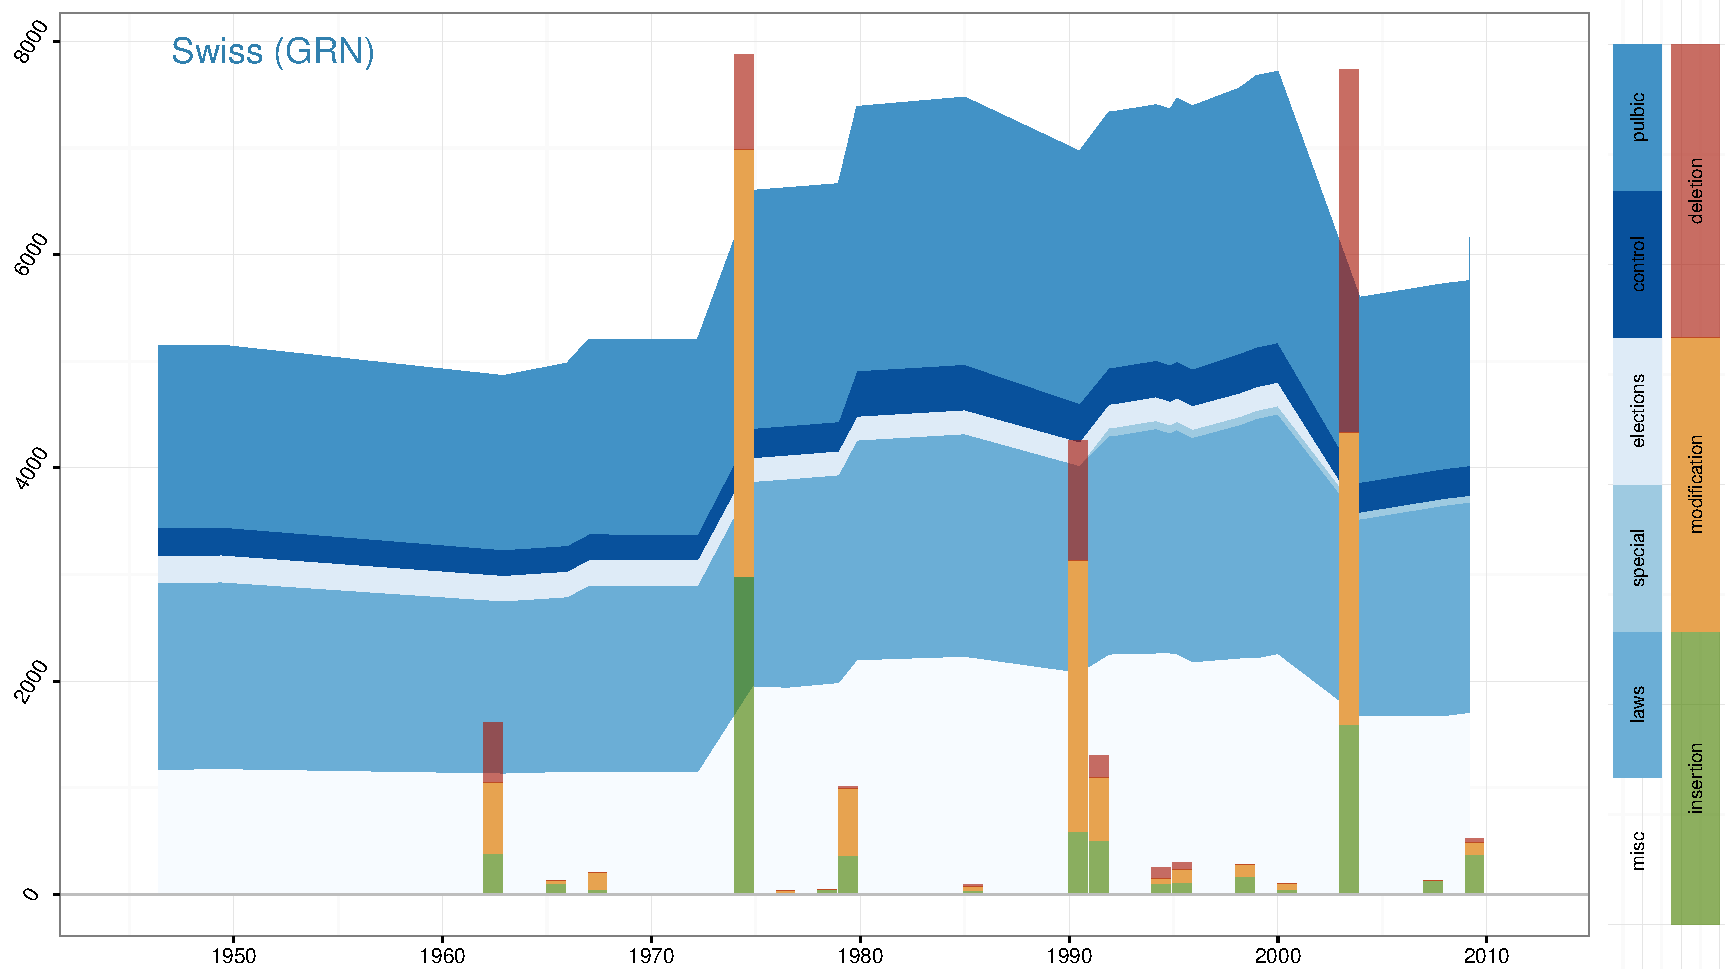
\includegraphics{country_graphs_files/figure-latex/unnamed-chunk-3-3.pdf}
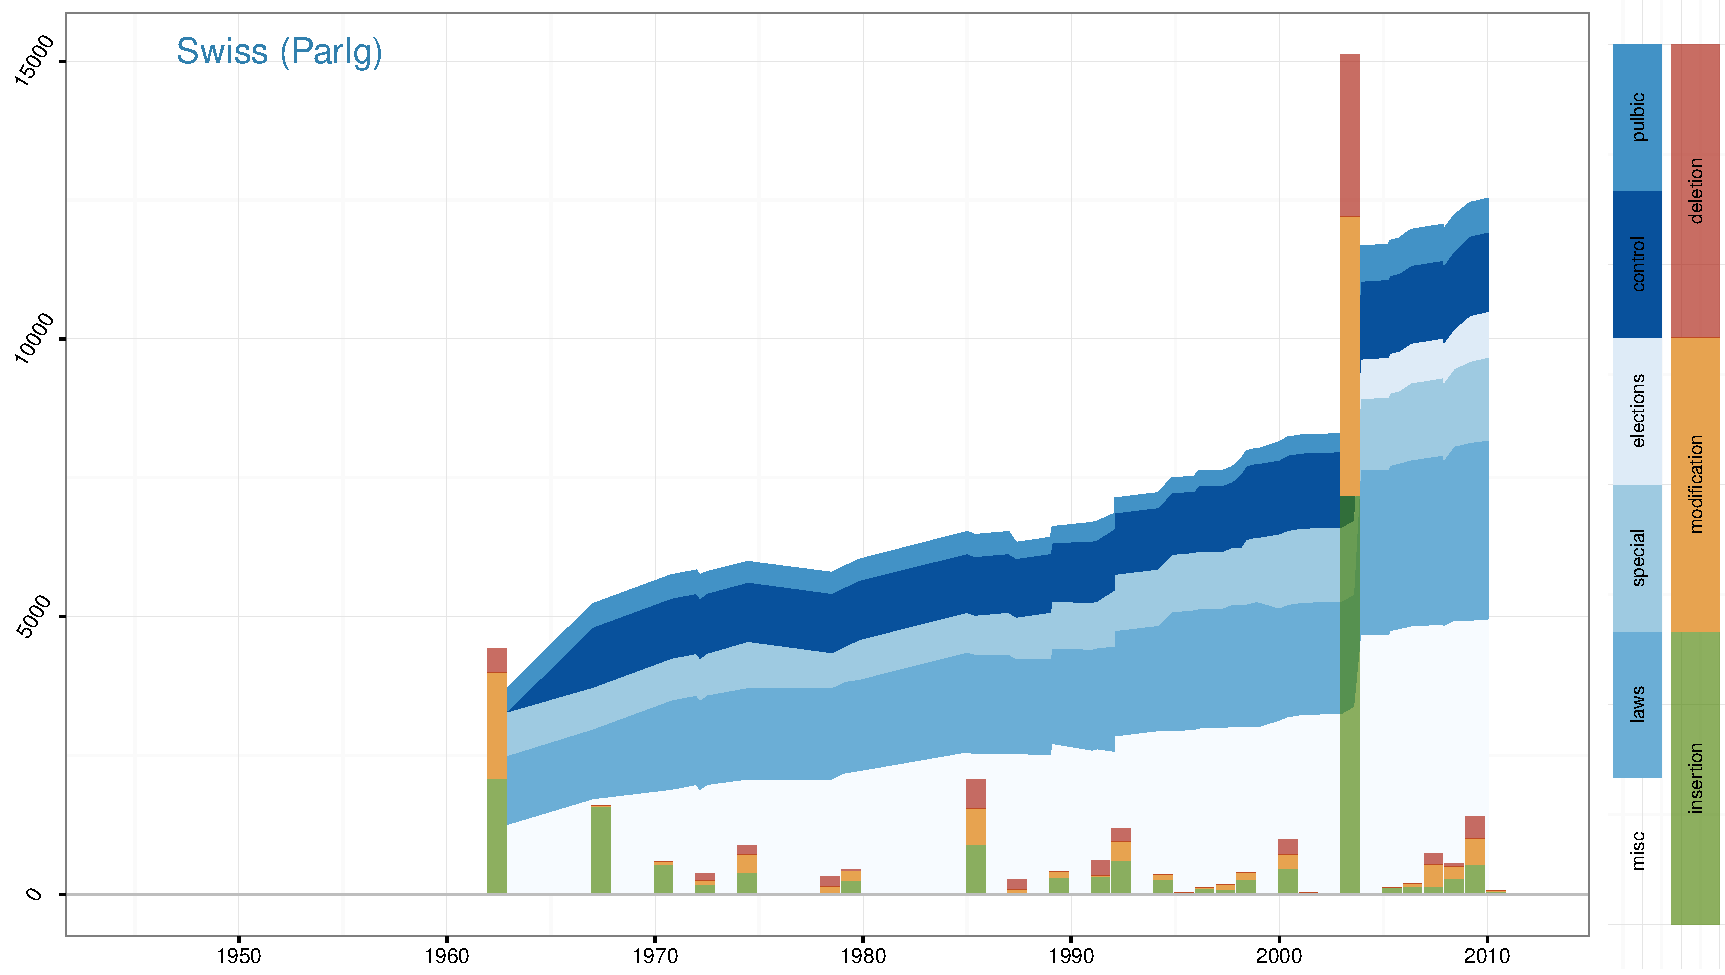
\includegraphics{country_graphs_files/figure-latex/unnamed-chunk-3-4.pdf}
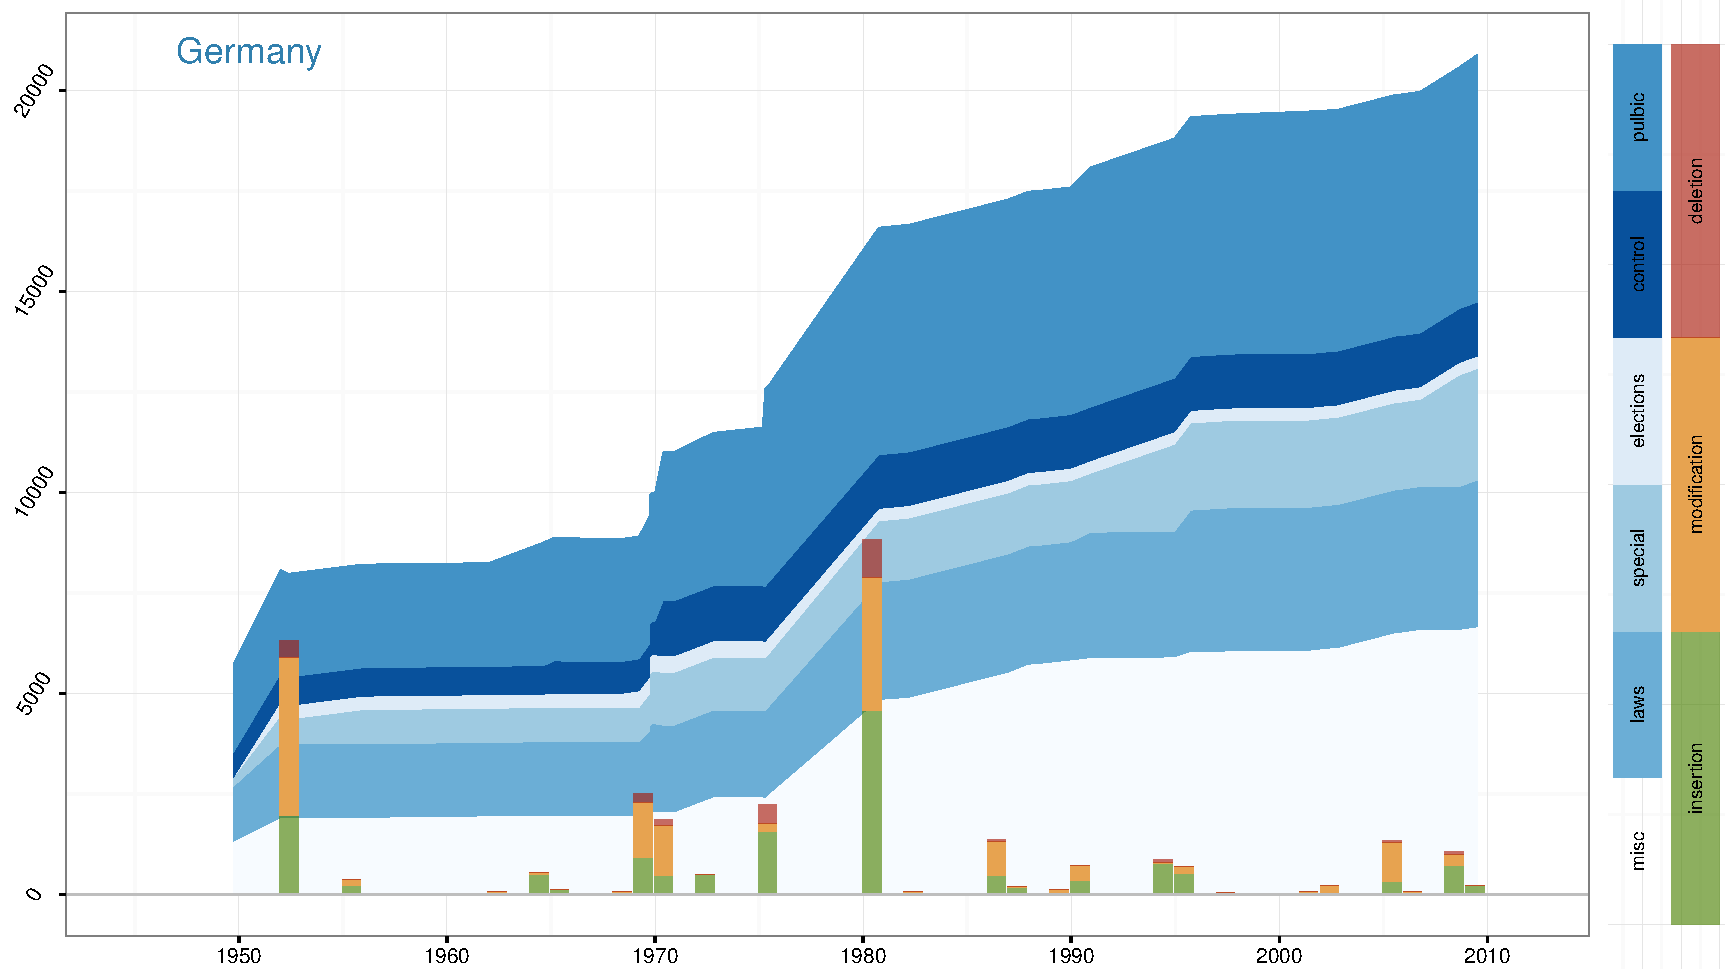
\includegraphics{country_graphs_files/figure-latex/unnamed-chunk-3-5.pdf}
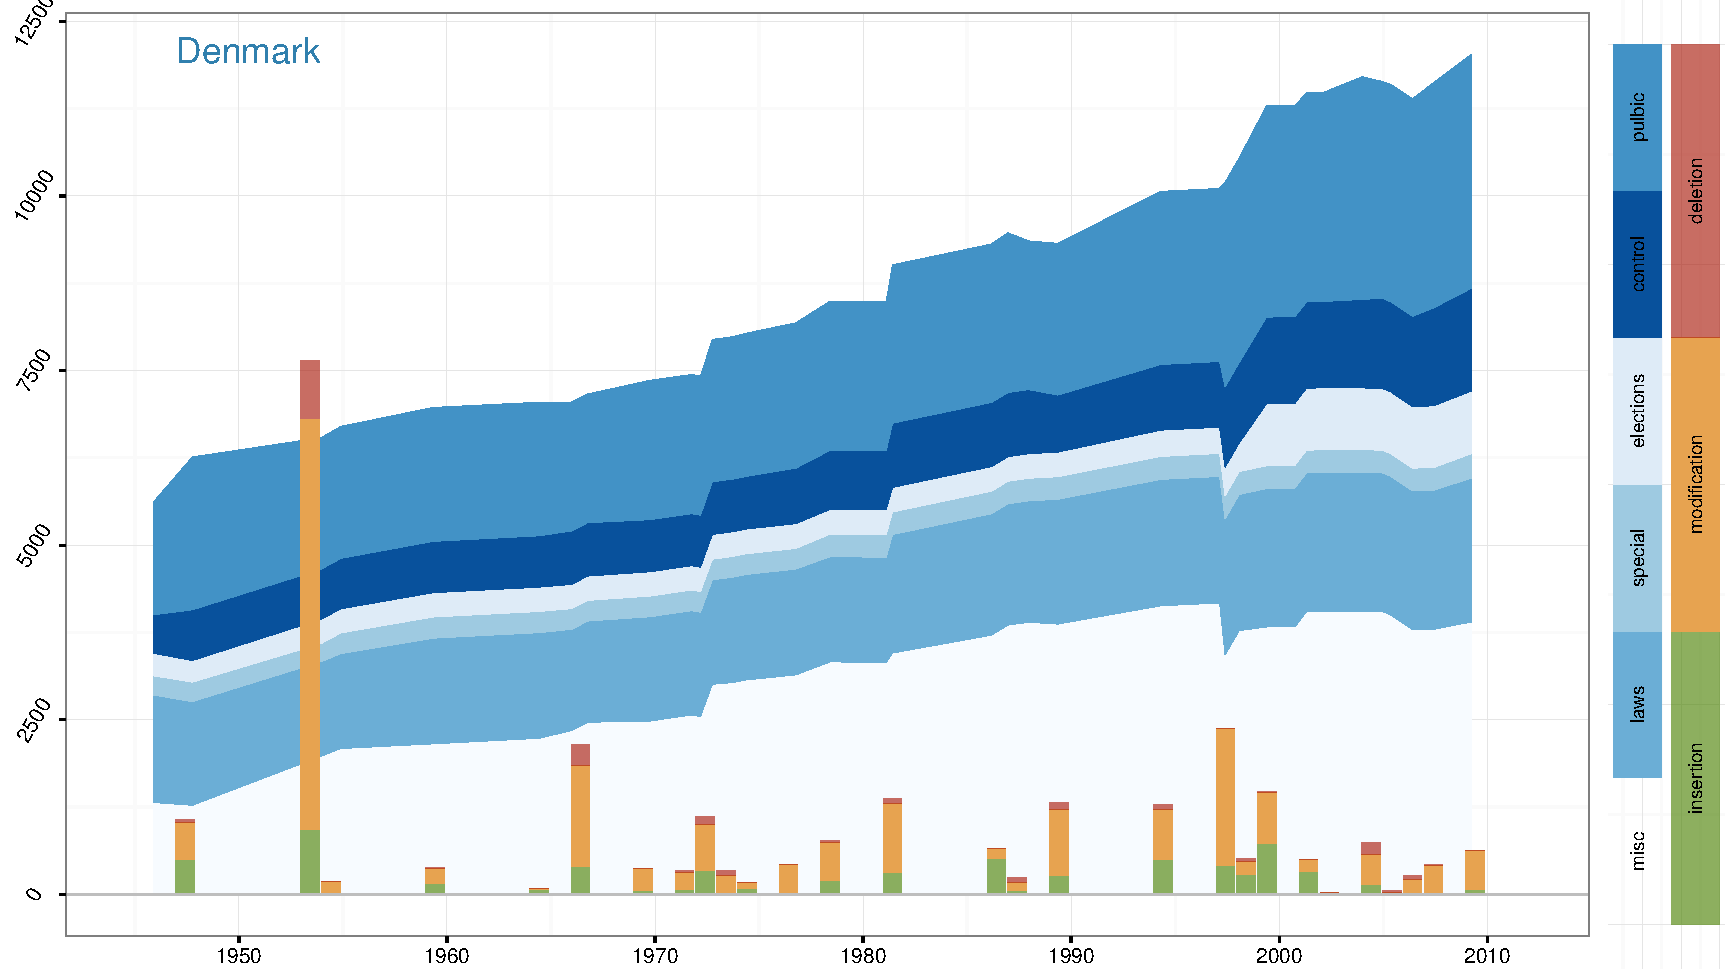
\includegraphics{country_graphs_files/figure-latex/unnamed-chunk-3-6.pdf}
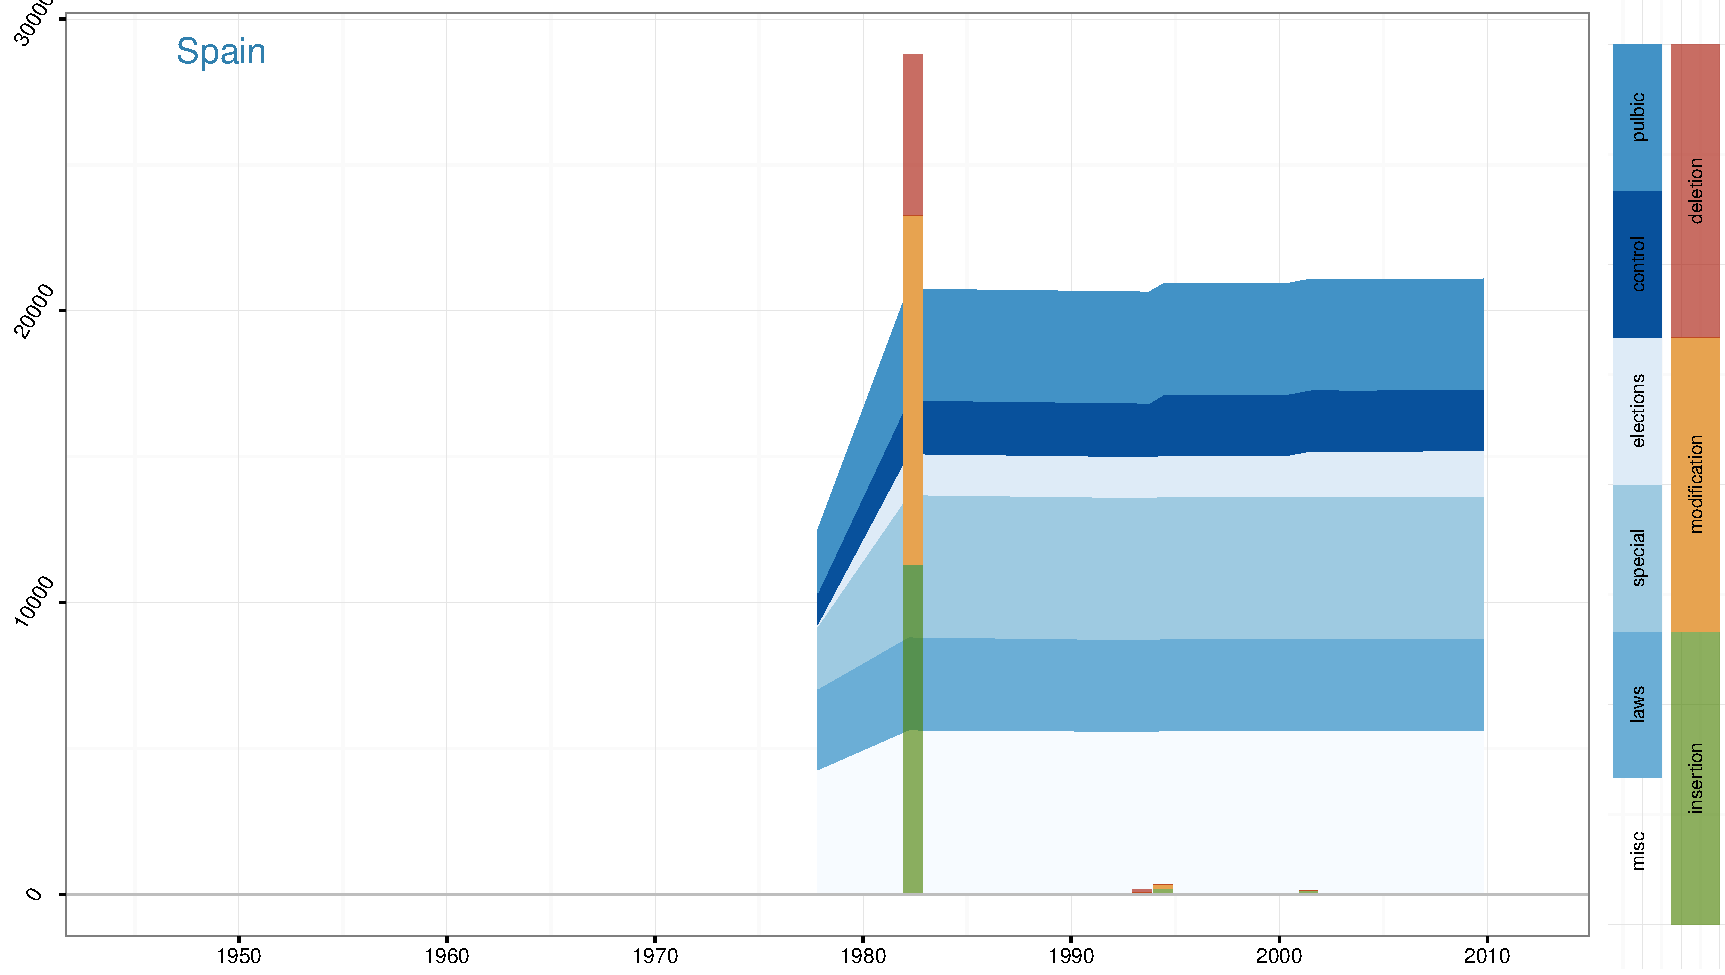
\includegraphics{country_graphs_files/figure-latex/unnamed-chunk-3-7.pdf}
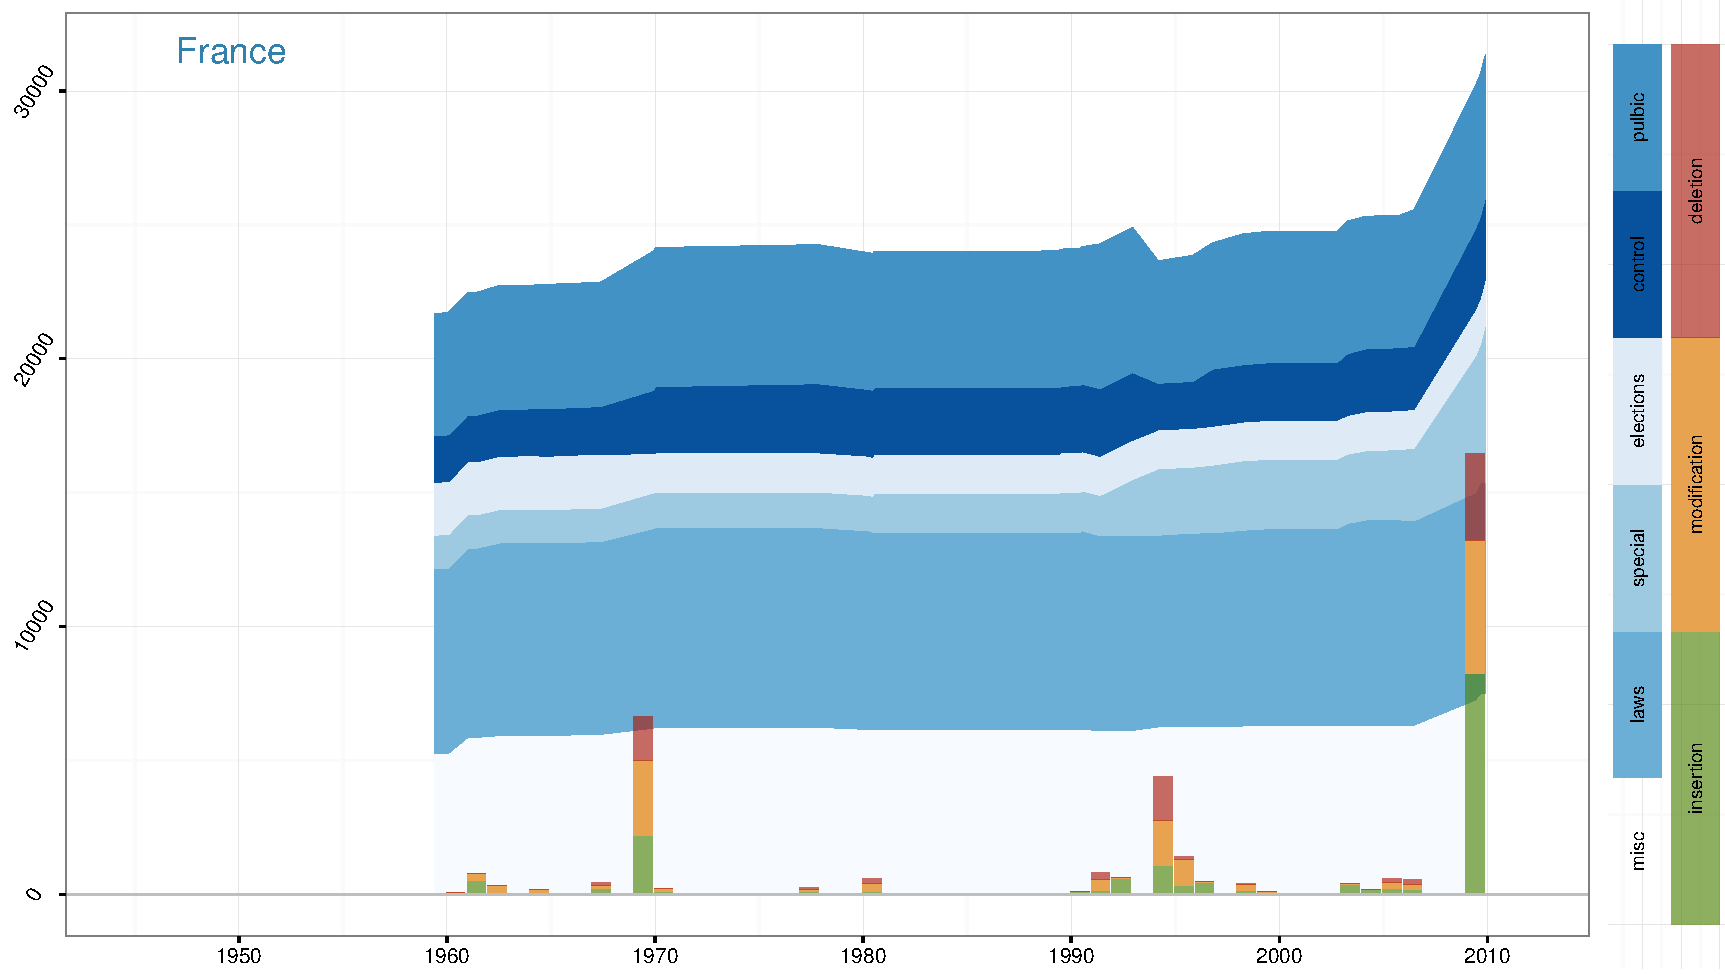
\includegraphics{country_graphs_files/figure-latex/unnamed-chunk-3-8.pdf}
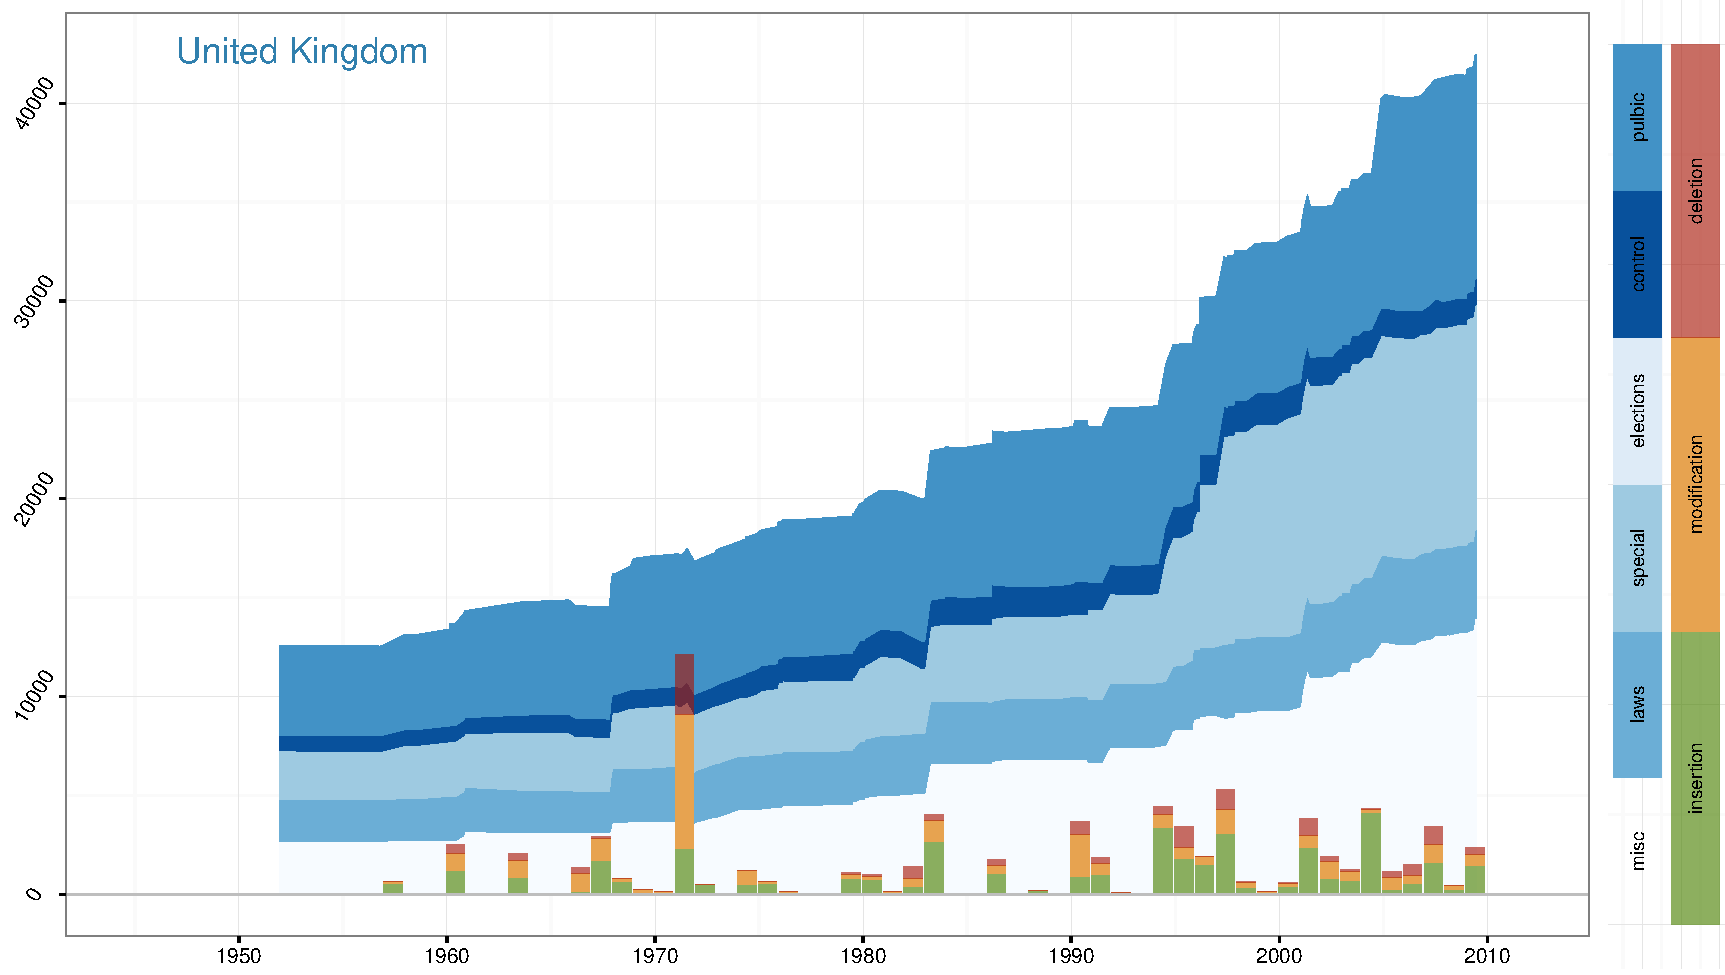
\includegraphics{country_graphs_files/figure-latex/unnamed-chunk-3-9.pdf}
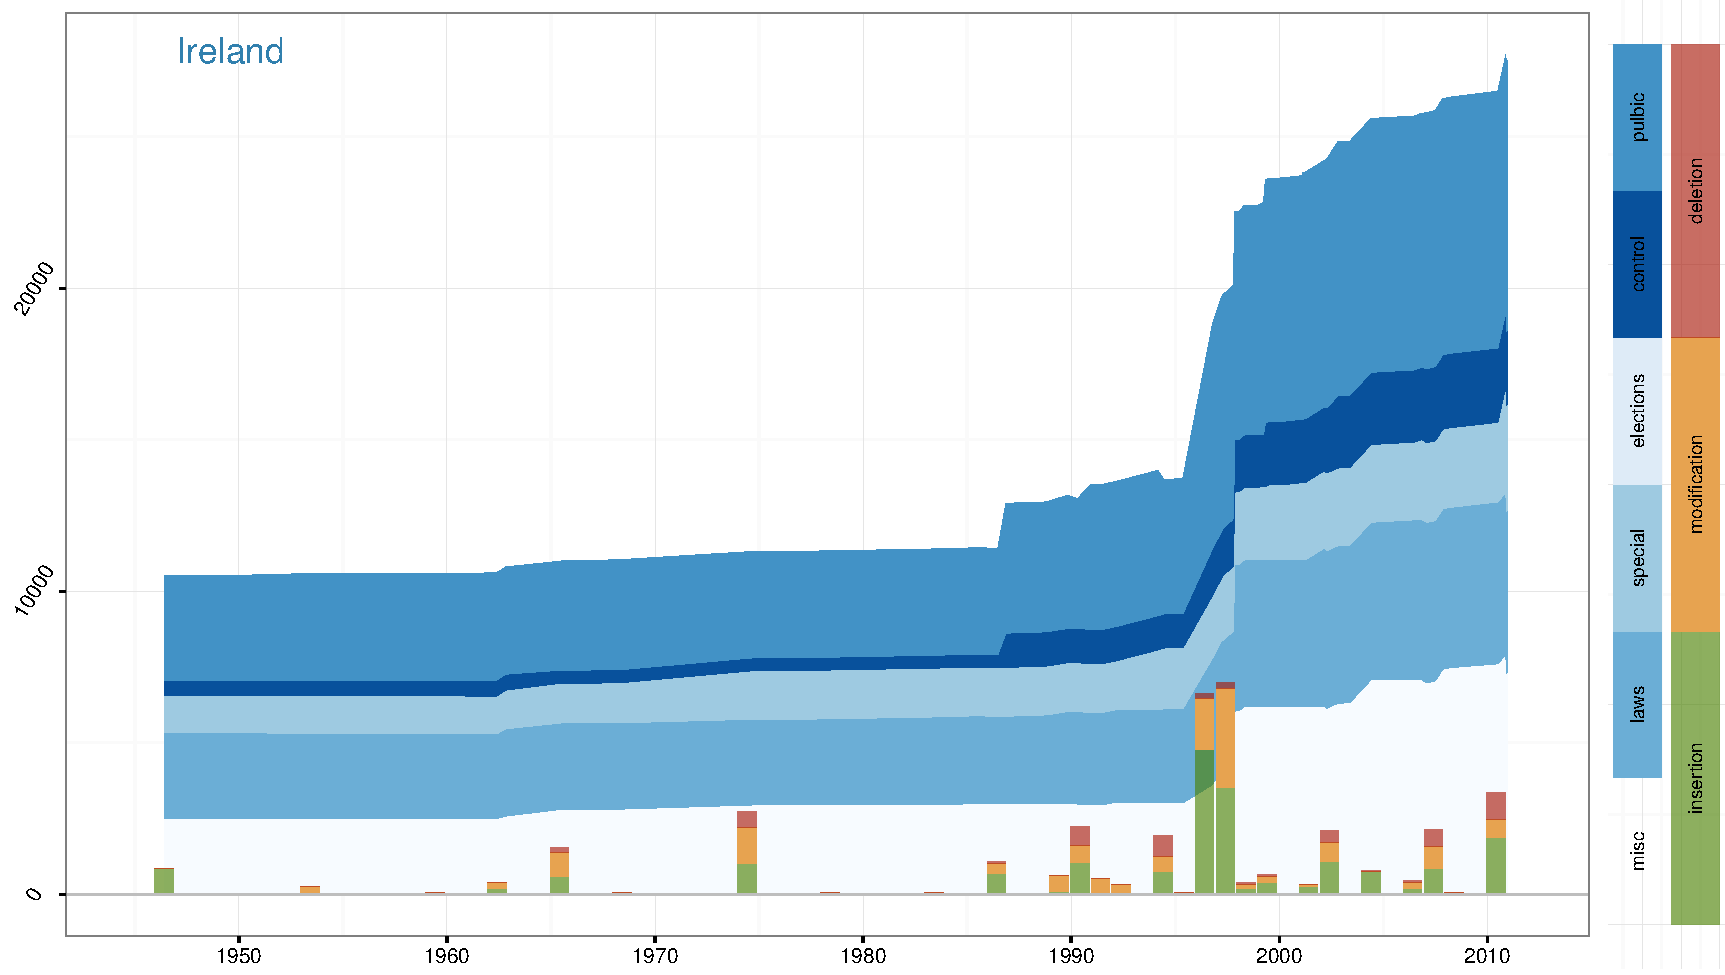
\includegraphics{country_graphs_files/figure-latex/unnamed-chunk-3-10.pdf}
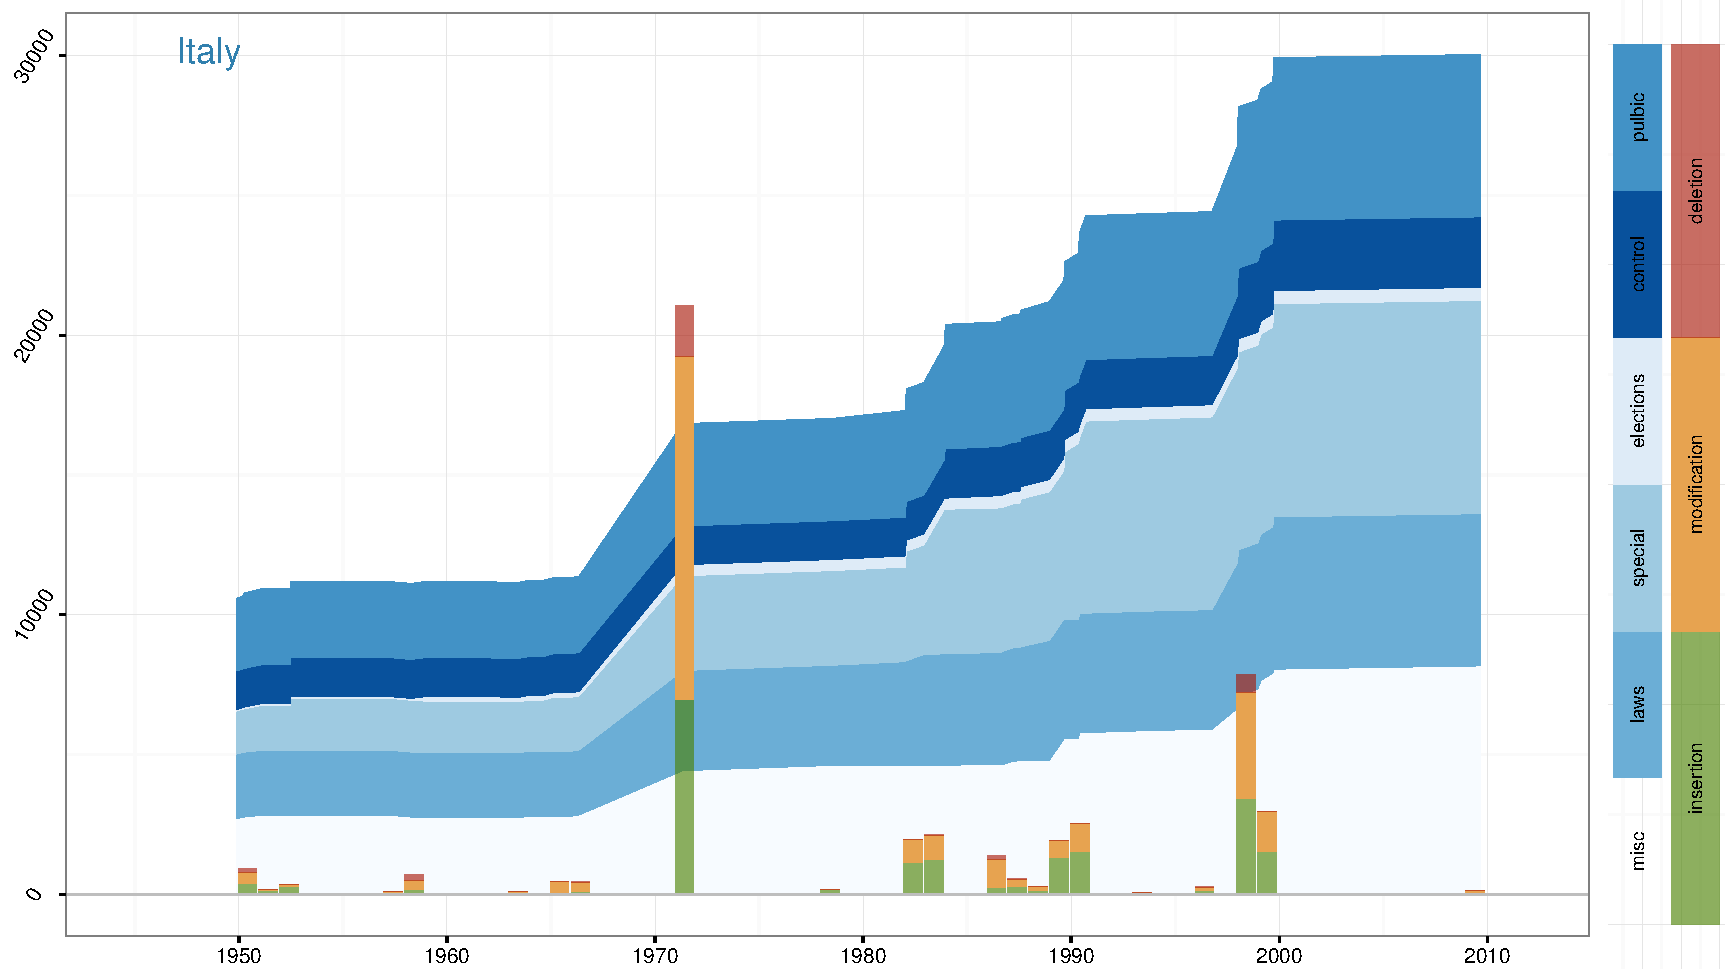
\includegraphics{country_graphs_files/figure-latex/unnamed-chunk-3-11.pdf}
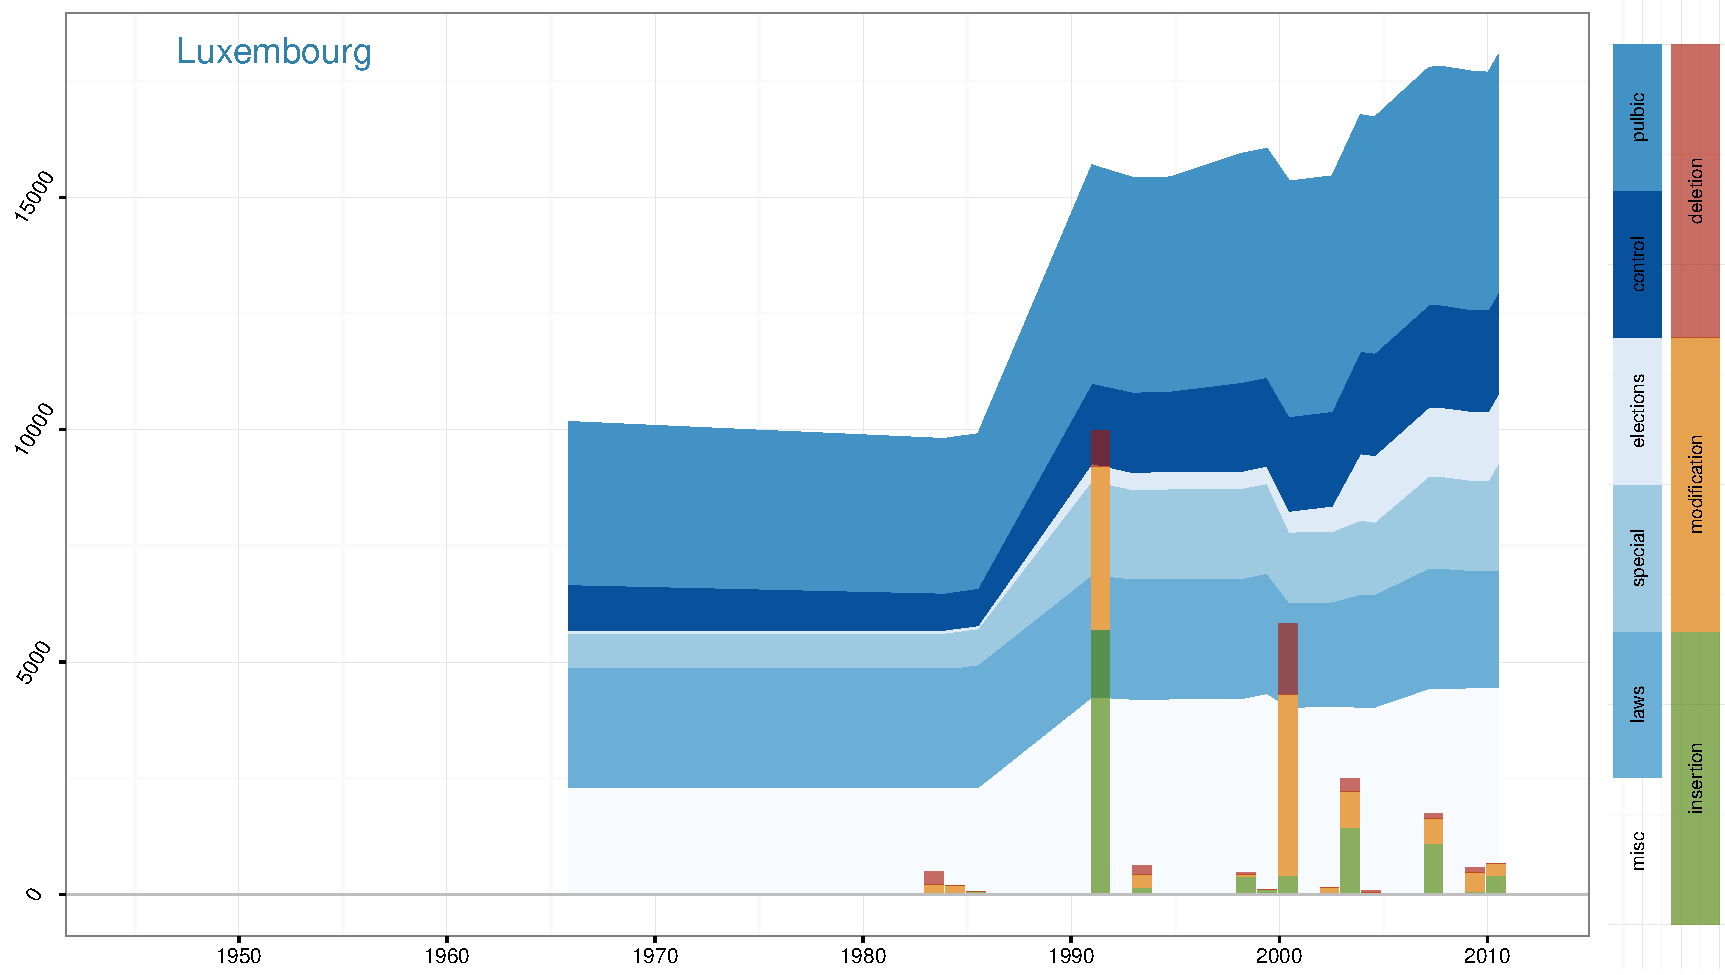
\includegraphics{country_graphs_files/figure-latex/unnamed-chunk-3-12.pdf}
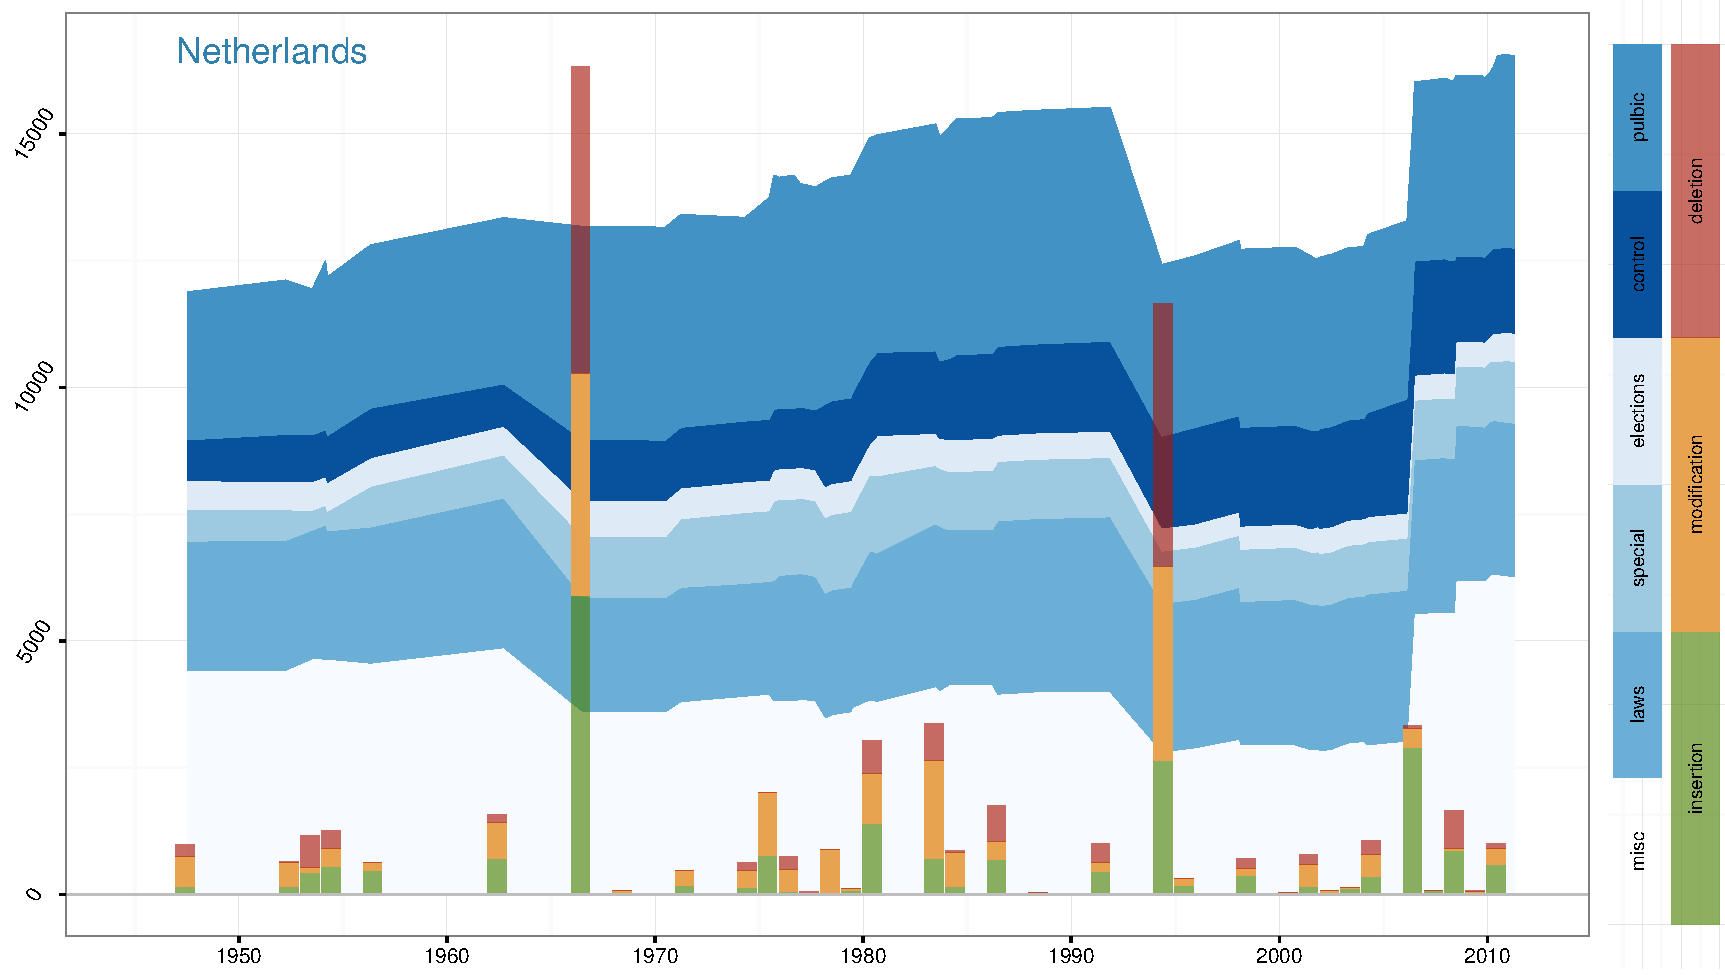
\includegraphics{country_graphs_files/figure-latex/unnamed-chunk-3-13.pdf}
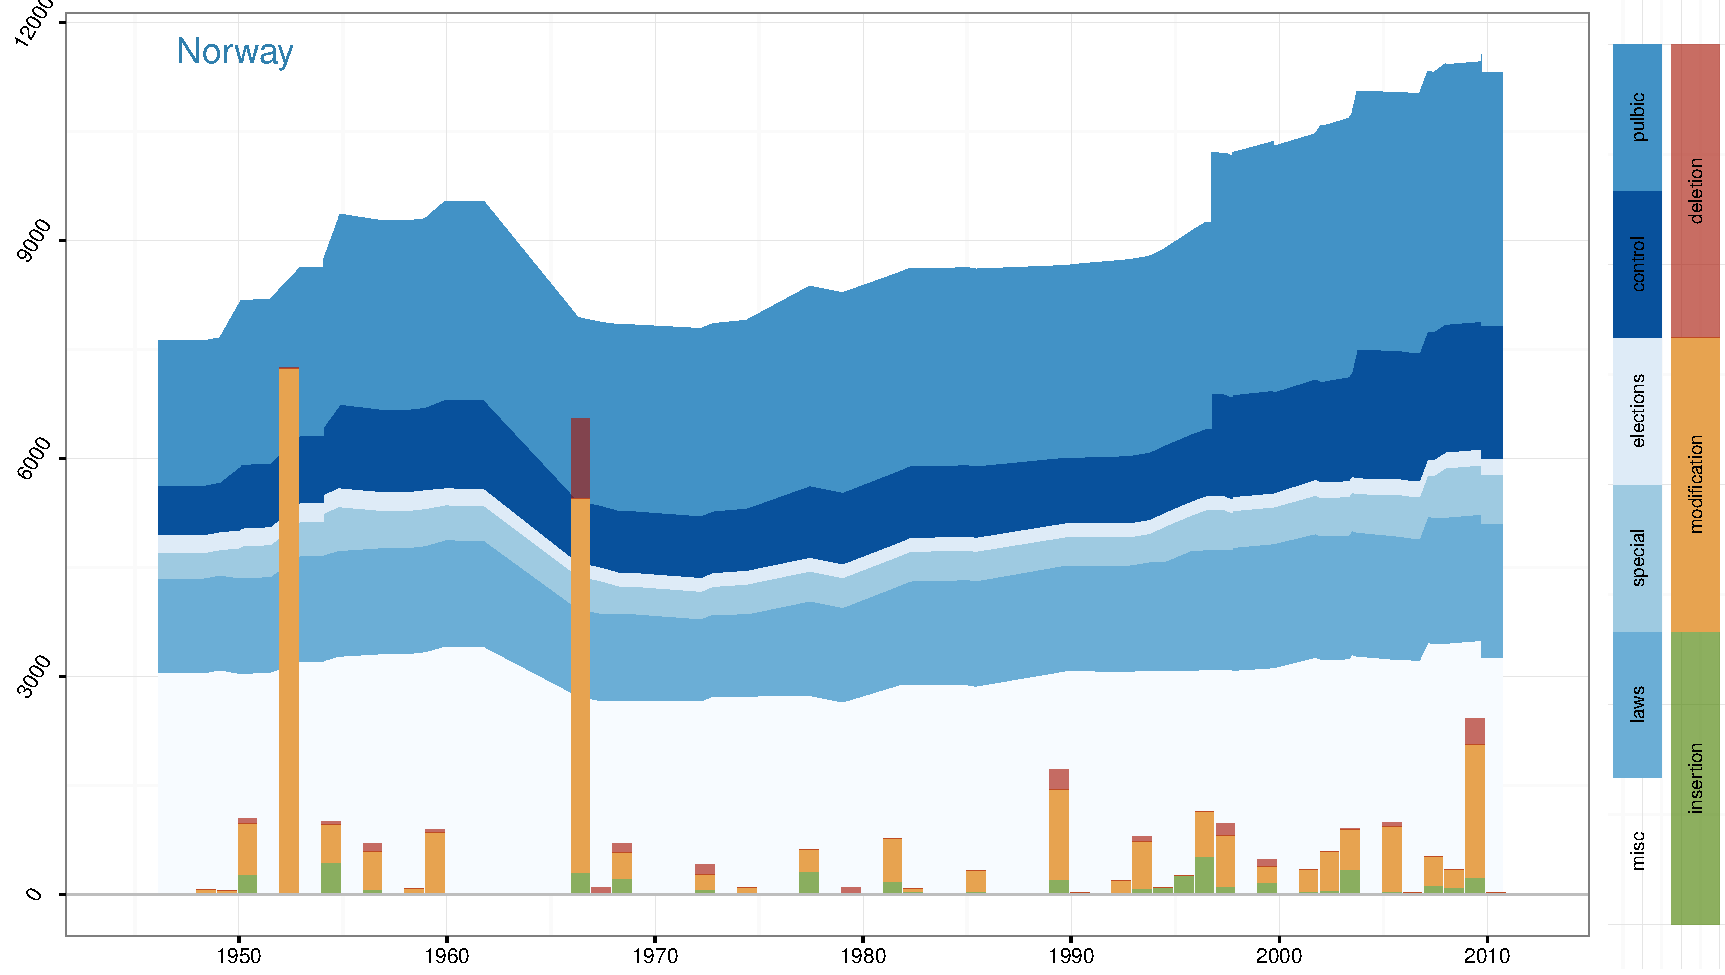
\includegraphics{country_graphs_files/figure-latex/unnamed-chunk-3-14.pdf}
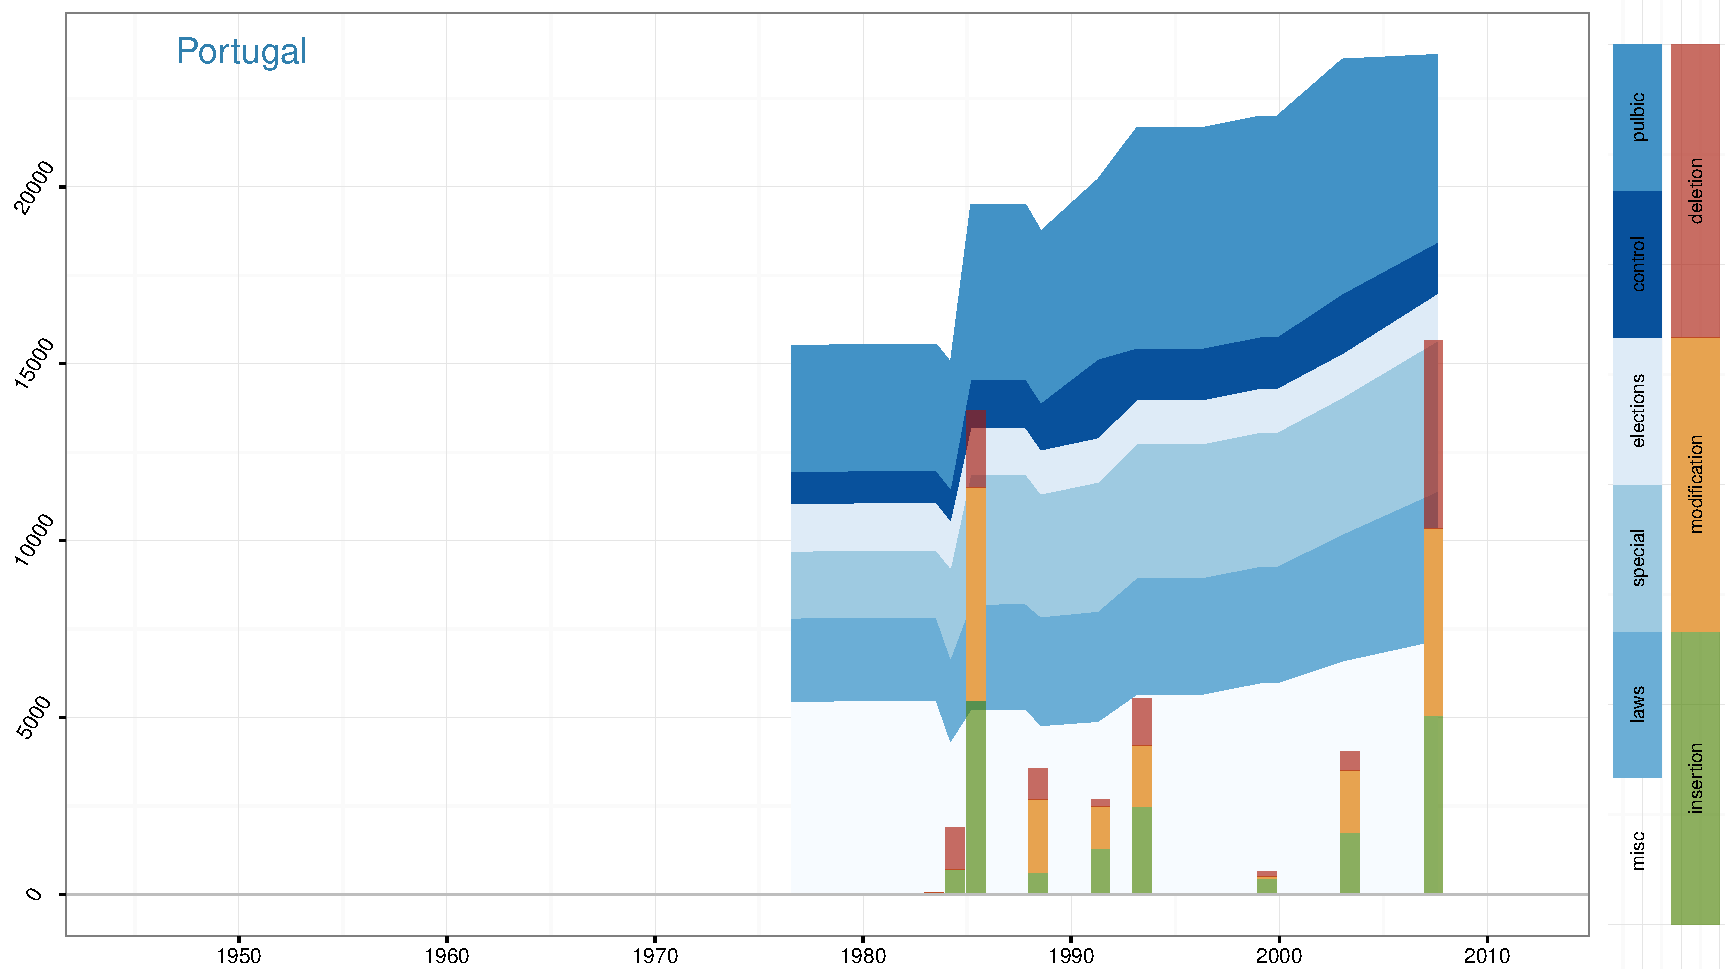
\includegraphics{country_graphs_files/figure-latex/unnamed-chunk-3-15.pdf}
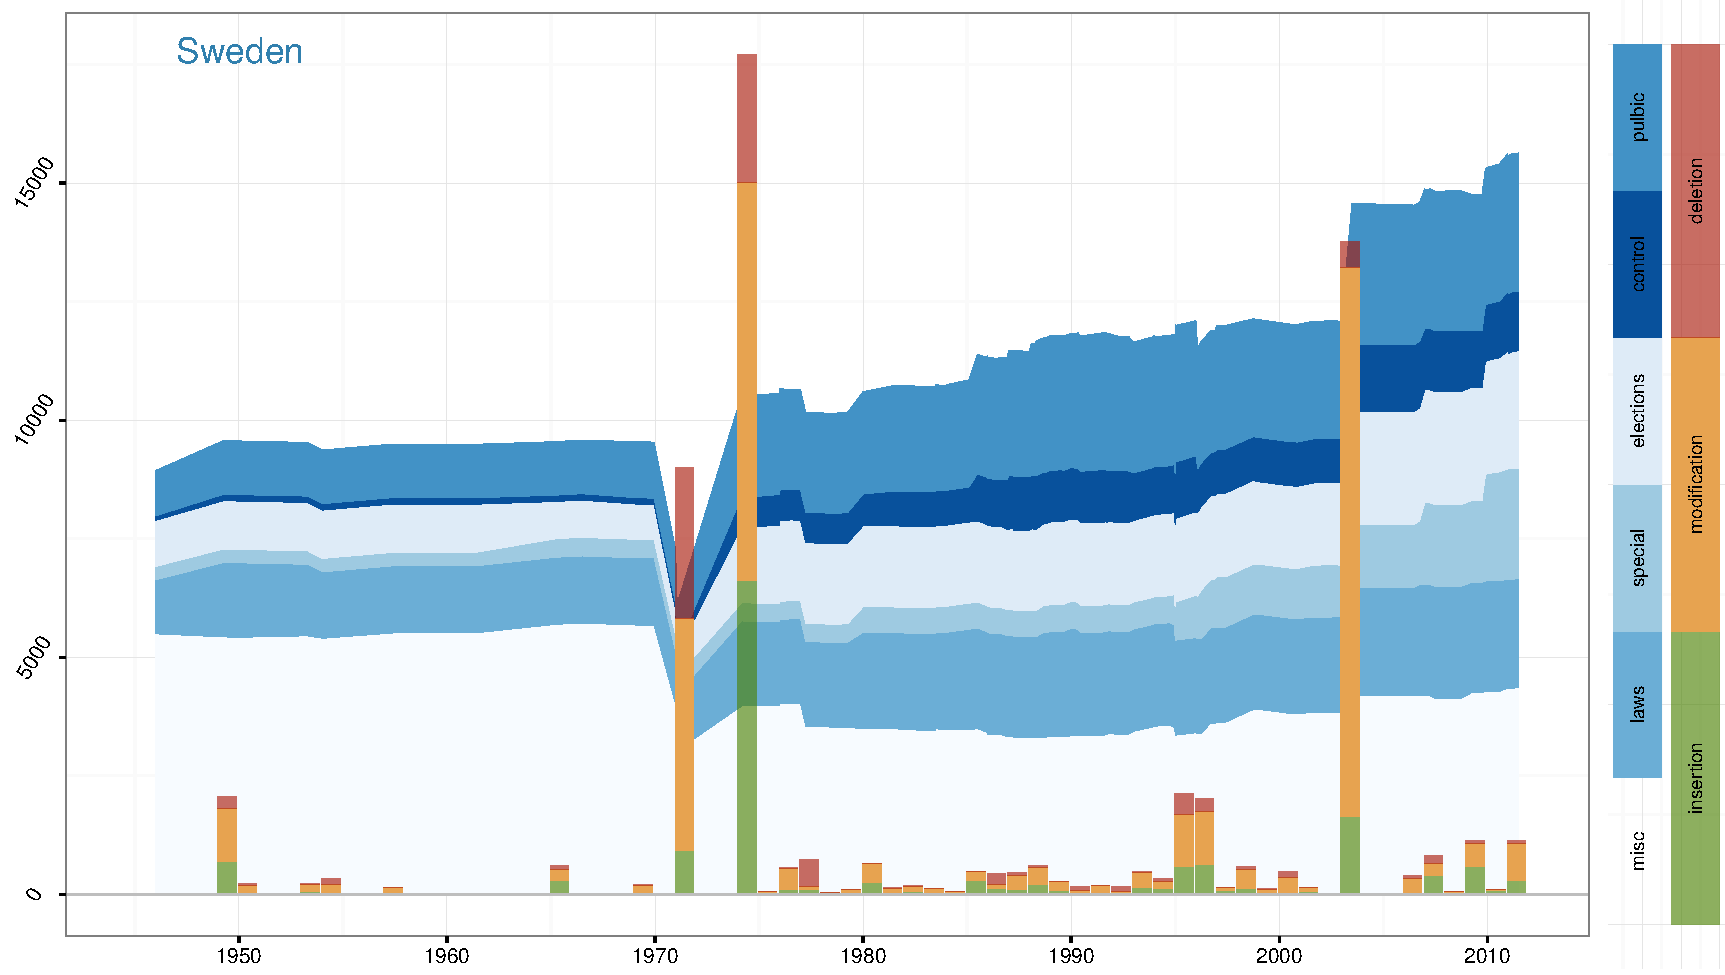
\includegraphics{country_graphs_files/figure-latex/unnamed-chunk-3-16.pdf}

\pagebreak{}

\section{dutiestodo}\label{dutiestodo}

\begin{verbatim}
## ==========================================================================
\end{verbatim}

\begin{verbatim}
## file copied to: 
## Z:/Geschäftsordnungen/Papiere und Konferenzen/2015_corpus_coding/in_progress/
\end{verbatim}

\begin{verbatim}
## [1] TRUE
\end{verbatim}

\end{document}
